\documentclass[uplatex,dvipdfmx,a4j,12pt]{jsarticle}

\usepackage[utf8]{inputenc}
\usepackage{graphicx}
\usepackage{amsmath}
\usepackage{comment}
\usepackage{color}
\usepackage{url}
\usepackage{siunitx}
\usepackage[version=4]{mhchem}
\usepackage{paralist}
\usepackage{longtable}
\usepackage{multirow}
\usepackage[dvipdfmx]{hyperref}
\usepackage{pxjahyper}

\usepackage{enumitem}
\setlist[description]{parsep=5pt}
\setlist[enumerate]{parsep=5pt}

% 半角文字のパーセント、より右側は、コメントとして扱われます。

% タイトルページの内容をここで記述します。
%
\title{
  「我が家のオーブンを用いた場合の\\    % \\ は、強制的に改行するコマンドです。
  マカロンの最適な焼き方」
  }
\author{
  金田 雅司 \\
  \\
  実験者番号: 0 \\
  }
\date{2025年 4月 1日}  % 提出日を記入して下さい


% ここから本文が始まります。
\begin{document}

% 上で設定したタイトルページの情報は、\maketitle があって始めて、コンパイル後に表示されます。
\maketitle

% レポートのフィードバックのコメントを希望しない場合には、
% 47行目から54行目までをコメントアウト(行頭に%を入れる)。
% コメントを希望する場合は、何について聞きたいかを具体的に書いて下さい。

% 縦方向の空白を挿入するコマンドです。em は行の高さ分、を意味する単位です。
\vspace{2em}
\begin{center}
    \begin{minipage}{0.5\linewidth}
        レポートのコメントを希望します。

        具体的には、方法の章で記述したことが、必要十分な情報になっているかどうか評価を下さい。
    \end{minipage}
\end{center}
\vspace{5em}  


% 概要は論文・レポート全体を一つの段落にまとめたものです。
% 物理の分野では、概要では段落分けをしません。
%
\begin{abstract}
    マカロンの焼き方について、オーブンの使い方が重要であるとの認識のもと、温度・時間の条件を変えて焼いてどのような焼き上がりになるかを調べた。
    その結果、我が家の電気オーブンレンジを使用した場合には、(1) 200℃で1分焼く、(2) 扉を開けず140℃に設定し引き続き3分焼く、(3) オーブンをオフにし5分おく、という焼き方が現状では最良であることが分かった。
    この手順で焼くと、表面にヒビが入らずピエもできると共に空洞が出来ていない。
\end{abstract}

% 強制的に改ページを行う
\newpage



\section{目的}

マカロンは人気のある菓子であり、人気パティシエ/パティエールの店で購入するだけでなく、手作りに挑戦する人もいる。
しかし、一般的に製菓はその作り方にコツ(あるいは経験の積み重ねによる感)が必要であると考えられている。

そのため、ウェブを検索すると様々なレシピのページ、および製菓過程の試行錯誤についてのブログ記事が見受けられる。
それらの記事から読みとれることは「マカロンが上手に焼けるようになるには自分の所有するオーブンのクセを見極めるのが重要である」と、いうことである。

つまり、温度コントロールがきちんと出来れば、上手に焼けると言える。
我が家のオーブンを使用した場合の最適な焼き方を得ることが、本研究の目的である。

ところで、この文章は、東北大学理学部物理学科の学部専門教育である物理学実験I のレポートを \LaTeX で書いてもらうための見本である。
章の書式、式・表・図のキャプションの書き方、参考文献リストの作り方等、文章の体裁に関することを一々考える必要がないため、\LaTeX を強く推奨する。

マカロンの研究において数式は出てこない。
そのため、\LaTeX を使うと美しい数式が書けることを以下に示す。
例えば、QCDのラグランジアン密度は、
\begin{equation}
    \mathcal{L}_\text{QCD} =\sum_\psi \left( i\bar\psi^j \gamma^\mu (\mathcal{D}_\mu\psi)_j -m_\psi\bar\psi^j \psi_j \right)-\frac{1}{4}G^a_{\mu\nu} G^{a\mu\nu}
    \label{eq:L_QCD} % label{ラベル名} を設定すると、\ref{ラベル名}で番号が自動的に参照される
\end{equation}
の様に記述することができる。
この式\eqref{eq:L_QCD} の美しさは、MS word や google document の数式モードでは実現不可能である。

Bessel関数の積分表示を書くと
\begin{equation*}    
    J_n ( z ) = \frac{ 1 }{ \pi i^n } \int_0^\pi e^{i z \cos \theta} \cos (n \theta) d\theta
\end{equation*}
であり、積分記号の傾きや大きさのバランスなど、ため息をつくほどの美しさである。

スピン0の相対論的な自由粒子の場を表すクライン=ゴルドン方程式も
\begin{equation*}
    \left [
        \frac{1}{c^2}\frac{\partial^2}{\partial t^2}
        - \nabla^2+\biggl ( \frac{mc}{\hbar} \biggr )^2
    \right ]
    \phi(\boldsymbol{x},t) = 0
\end{equation*}
の様に書くことができる。



\section{方法}

この章では、マカロンの材料と配合、仕様した道具、作成手順、焼き方について述べる。


\subsection{マカロンの材料と配合}

今回用いたマカロンの材料の配合を、表\ref{table:recipe}に示した。
この配合は、cuocaのレシピ(参考文献\cite{cuoca}
\footnote{
    cuocaは、2017年に富澤商店に事業譲渡された(参考文献~\cite{cuoca-tomiz})。
    cuocaのWebページはしばらくそのまま残っていたが、今は消えている。
    そこに載っていたレシピは、富澤商店のページに掲載されており、参考文献\cite{cuoca}のものは、参考文献\cite{tomiz}として閲覧可能である。
}
)を元にしている。 
なお、このレシピでは、フレンチ・メレンゲ
\footnote{
    卵白に砂糖を少しずつ足しながら泡立てたもの。これに対して、砂糖に少量の水を加えて火にかけ、118℃まで煮詰めたシロップを卵白に少しずつ足しながら泡立てたものをイタリアン・メレンゲと呼ぶ。
}
を用いている。 

なお、参考文献~\cite{cuoca}にあるレシピの分量と比べると乾燥卵白の分量が異なっている。 
これは、我が家にある電子秤の目盛りが 1g 単位であるため、元のレシピが有効数字2桁に対し、この実験では有効数字1桁でしか計測出来なかったためである。

\begin{table}[t]
    \centering
    \caption{マカロンの材料。作成の際に使う順番に並べてある。乾燥卵白以外はスーパーの製菓コーナーでよく見かけるものである。}
    \begin{tabular}{lr}
        材料              & 質量 \\
        \hline
        グラニュー糖      & 17g \\
        乾燥卵白         & 3g \\
        卵白             & 50g \\
        アーモンドプードル & 50g \\
        純粉糖 & 90g \\
        \hline
    \end{tabular}
    \label{table:recipe}
\end{table}

\subsection{材料の入手方法}

レシピにある材料のうち、乾燥卵白は cuoca で購入していたもの(乾燥卵白20g)を用いた。
なお、仙台では、乾燥卵白はサトー商会の店舗で購入できる。
グラニュー糖および卵白は近所のスーパーマーケットで購入して家にあったものを使用した。 
アーモンドプードルと純粉砂糖は、サトー商会の店舗で購入した。

表\ref{table:recipe}に記載している以外の材料として、ピンクに着色するため食用色素(赤)を用いた。
この食用色素は、家のキッチンにストックしているものを用いたが、スーパーの製菓材料コーナーに行けば通常手に入るものである。

\subsection{道具}

\begin{table}[t]
    \centering
    \caption{必要な道具のリストを示す。元のレシピにはメレンゲの泡をつぶす時にカードを使うとあるが、ゴムべらで良い。}
    \begin{tabular}{lc}
        道具名              & 数量 \\
        \hline
        ステンレスのボール      & 1 \\
        ハンドミキサー(電動泡立て器) & 1 \\
        ゴムべら(シリコーン製が使いやすい)  & 1 \\
        絞り袋 & 1 \\
        直径8mmか10mmの口金 & 1 \\
        クッキングシート & 1 \\
        オーブン & 1 \\
        \hline
    \end{tabular}
    \label{table:tools}
\end{table}

必要な道具を表\ref{table:tools}にまとめた。
これは、製菓を趣味としている人手あれば、通常キッチンに常備してあると思われる一般的な道具である。
道具の選定についても、以下に記録を残こす。

製菓の場合、ボールはステンレスが良い。
これは、色々なお菓子を作る場合、その行程で、火にかけたり、湯煎にかけたり、氷水で冷やしたりすることがあるため、熱伝導がよく丈夫でさびないステンレス製一択である。

cuocaのレシピでは、メレンゲの泡をつぶす際により大きなボールに移してカード
\footnote{
    あるいは、スケッパー、ドレッジと呼ばれる道具。
    ボールの側面にピッタリ着くように弧を描いている大きめのヘラ。
}
を使うとある。
まず、洗い物を増やしたくないので、ボールは一つしか使わなかった。
カードはあれば便利だが、使わなくてもゴムべらでメレンゲの泡はつぶせる

絞り袋や金口も、製菓道具店(もしくはWebの通信販売)で購入可能である。
これも仙台ではサトー商会で買える。

クッキングシートは、スーパーの製菓道具コーナーで購入可能である。
か、店によってはアルミフォイルや食品用ラップ(いわゆるサランラップ)のコーナーに置いてある。

この実験で用いた、電気オーブンは、Natioal
\footnote{
    松下グループ(現在のパナソニック)のブランドの一つ。
    2008年にブランドが消失した。
    今の大学生の年では「生まれていない」ほど昔ではないが、ナショナルを知らない人が多いのではなかろうか。
    筆者にとっては、光陰矢のごとしである。
}
の NE-F3である。 
実験を行った2012年10月時点で、購入後7年近く経っているがまだ現役で活躍していた。

\subsection{作成手順}

マカロンの作成手順については、参考文献\cite{cuoca}に掲載されているものに従った。
なお、再現実験を試みる方の為に、手順の中で注意すべきことを以下に述べる。

(1) メレンゲの作成には泡立て器は手動ではなく電動のものを使う。
(2) 全ての材料を混ぜた後にメレンゲの泡をつぶすが、スポンジケーキの作成の経験が有る場合はその感覚に引きられると、つぶし方が足りない状態になり、焼いたときに膨らみ過ぎになる。

クッキングペーパーの上に絞った(図~\ref{fig:fig01}参照)後、表面が十分乾燥するまで待った。 
今回の実験では、室温23℃ 湿度60\%で約2時間弱待機していた。
%  % を文字として使いたい場合には、半角のパーセントの前にバックスラッシュ(環境に依っては半角の円マークに見える)を入れる。

\begin{figure}[b]
    \centering
    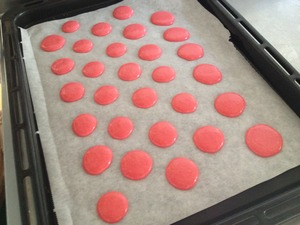
\includegraphics[width=0.5\linewidth]{fig01.jpg}
    \caption{クッキングペーパーにマカロンの生地を絞った直後の写真。乾燥させる前なので、生地の表面につやがある。}
    \label{fig:fig01}
\end{figure}

マカロンは、生地をつくり天板に絞った後、表面を乾燥させる作業が必要となる。
本来は、乾燥場所の気温と湿度を記録し、乾燥時間をどのくらいにするかも、マカロンの焼き上がりに重要なパラメータとなる。

良い焼き上がりのマカロンにするためには、乾燥後表面を指でそっと触って、生地が手に着かず、適度に結晶化している状態が良い。
この状態を達成するには、実験を行った10月の時点で我が家のキッチンで2時間弱乾燥させれば良いことが予備実験によって分かっている。
そのため、今回は乾燥を行う条件について、パラメータの最適化は行わなかった。

表面を乾燥(今回は2時間弱かかった)させた後に、絞り出した生地一つずつ焼き方の条件を変えて焼き上がりの状態がどのようになるかを調べた。

\subsection{焼き方}

オリジナルのレシピでの焼き方は以下の通りである。
\begin{itemize}
    \item 210℃ に余熱したオーブンの中段に入れ三分焼く。

    \item ピエが出来たら140℃ に下げて約7~8分焼く。
    \item 温度を下げるときに扉は開かない。    
\end{itemize}
なお、ピエとはマカロンを焼き上げたときに、天板の接した場所にできるギザギザ状のものを指し、フランス語の足 (= pied) である。

温度を一気に下げるにはオーブの蓋をあける必要がある。
しかし、どのくらいの時間あけるのか、外気温が何度なのかによって、完全にコントロールするのは難しい。
そのためこの実験では、オリジナルのレシピにある「140℃に下げて約7〜8分焼く」という部分を、「140℃に設定して約7〜8分焼く」とした。

この方法をとった場合に、予想されるのは焼きすぎになるだろう、ということである。
そのため、最初その予想通りになるかを確認した後、オリジナルの焼き方から少しずつ変え、できあがりを比較することとした。
その組みあわせについては、次章で述べる。


\section{結果}


\begin{table}[t]
    \centering
    \caption{焼き方と焼き上がりの関係を調べるために、条件を変えてマカロンを焼いた。四回目と五回目では「焼き時間2」の後、それぞれ3分と5分それぞれ放置した}
    \begin{tabular}{cccccc}
    	&       & 最初の   &         & 次の     &  \\
        & 天板の & 温度設定 & 焼き時間1 & 温度設定 &焼き時間2 \\
        & 位置 & [℃]    & [分]     & [℃]   & [分] \\
        \hline
    一回目 &	下段 & 210 & 3 & 140 & 7 \\
    二回目 & 中段 & 210 & 1 & 140 & 8 \\
    三回目 & 中段 & 210 & 1 & 140 & 5 \\
    四回目 & 中段 & 200 & 1 & 140 & 4 \\
    五回目 & 中段 & 200 & 1 & 140 & 3 \\
        \hline
    \end{tabular}
    \label{table:combination}
\end{table}

\begin{figure}[b]
    \centering
    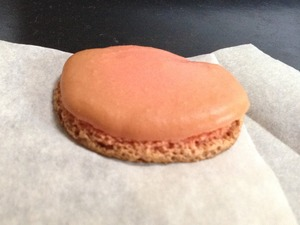
\includegraphics[width=0.22\linewidth]{fig02.jpg}
    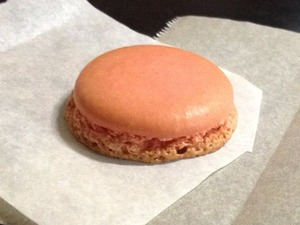
\includegraphics[width=0.22\linewidth]{fig03.jpg}
    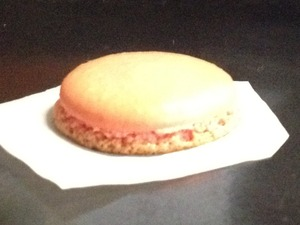
\includegraphics[width=0.22\linewidth]{fig04.jpg}
    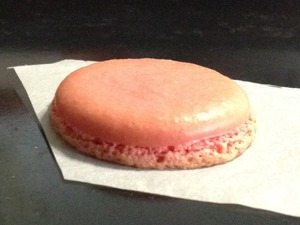
\includegraphics[width=0.22\linewidth]{fig05.jpg}
    \caption{一回目(左端)から四回目(右端)までの焼き方のテストでのマカロンの焼き上がりの写真。}
    \label{fig:fig02}
\end{figure}

実際に試した組みあわせを表~\ref{table:combination}にまとめた。
表の項目の「最初の温度設定」は、マカロン生地が乗った天板を入れる前に余熱で温めていた温度である。
その温度の状態で、生地の乗った天板をオーブンに入れ、「焼き時間1」の時間をセットしスタートボタンを押した。
時間が経ちストップすると、温度の維持は止まる。
オープンの扉は開けず「次の温度設定」の温度に設定し、「焼き時間2」の時間をセットしスタートボタンを押し、時間が経ちストップしたあと、天板を外に出した。

一回目(図~\ref{fig:fig02}の左端の写真)では、ピエは形成されたが、膨らみ過ぎで表面が剥離しかけている結果となった。
また、表面に焼き色が付いた。

二回目(図~\ref{fig:fig02}の左から二番目の写真)では、表面の剥離はしていないが、焼き色がついている。

三回目(図~\ref{fig:fig02}の左から三番目写真)では、少し焼き色がついている。
写真を撮る際に被写体が他の写真のマカロン撮影時よりも遠くにあったため撮影条件が悪く、残念ながら目で見た色が写真では再現されていない。

四回目(図~\ref{fig:fig02}の右端の写真)のテストの結果では、マカロンの形状、ピエの出来方は満足出来たが、心持ちうっすらと茶色っぽい。 
そのため、理想にはもう一歩という印象を受けた。
四回目では、「焼き時間2」は他のよりも短くし、温度維持が終わったあと3分放置している。
これは、140℃から少しずつ温度が下がっていく状態で、結果がどうなるかを調べるためである。

五回目では、「焼き時間2」を一分短くし、オープンの中に放置しておく時間を2分長くした。
焼き上がりはこの条件がベストであっった。

なお、各回とも、最初にマカロンをオーブンに入れてから1分30秒後にピエが形成され始めた。

% LaTeXには、幾つかの単位がありますが、 \linewidth は、その文章のスタイルで
% テキストが書かれる場所の横幅の変数として定義されているものです。
% cm で絶対値を指定することも出来ますが、\linewidth を使うと相対値として指定出来ます。
\begin{figure}[b]
    \centering
    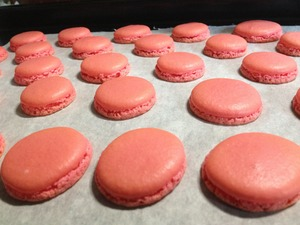
\includegraphics[width=0.6\linewidth]{fig06.jpg}
    \caption{最終的な焼き時間として採用したマカロンの焼き上がりの写真。五回目の焼き方で焼いたものである。}
    \label{fig:fig06}
\end{figure}

\section{考察}

条件を少しずつ変えながら焼いた。
焼く温度と焼く時間に対する焼き上がり具合から、次に焼く条件を試行錯誤した。
そのため、各回に対してどのように考察して次の実験条件を設定したかについてをこの章で記述する。

一回目の結果では、表面が剥離しかけるくらい膨らみ過ぎであった。
これは、下段に天板を置いても与えられた熱量が多すぎることを意味する。
そのため、二回目ではレシピ通り天板は中段に置いてテストすることにした。
そして「焼き時間1」を短くし、「焼き時間2」をその分長くして試すことを考えた。

二回目では、表面の剥離は無かった。
これは、予想通り最初の高温の設定を短くしたことが良かった考えられる。
一方、焼き色が付いたことは焼き上がるまでに加えた温度が高いことを意味する。
そのため三回目では、「焼き時間2」を二回目よりも短くした。

三回目でもまだ焼き色が付いたため、最初に加える熱量を少なめにした方が良いと判断した。
そのため、四回目では「最初の温度設定」を200℃に変え、「焼き時間2」も短くし、その後オーブンの温度が徐々に下がっていく状態で3分経ったところで取り出した。

四回目では、理想的なマカロンの焼き色には今一つという結果であった。
そのため、「焼き時間2」をさらに短くし、オーブン内に放置する時間を長くすることで、理想的な焼き色になると予想した。

\section{結果}

この実験の結果、以下の事が判明した。
\begin{itemize}
    \item 天板の位置はオリジナルのレシピ通り中段で良い。
    \item オリジナルのレシピ通りに焼くとこのオープンでは焼きすぎになり、膨らみ過ぎによる表面剥離及び薄茶色の焼き色がついた。
    \item このオーブンは温度が高い状態から低い状態に設定を変えると、自然に温度が下がるまで待つ。熱排出及び冷気送風などにより一気に温度が下がることはない。そのため「途中で温度を下げる」レシピはそのまま採用できない。
\end{itemize}

最終的に採用した焼き方は以下のものである。
\begin{itemize}
    \item 天板はオーブンの外に出して置き室温の状態でマカロンの生地を絞ったクッキングペーパーを乗せる。
    \item 中段を使用。
    \item 200℃に暖めたオープンで1分焼く。
    \item 1分経過後、扉を開けず140℃3分に設定し引き続き焼く。
    \item 3分経過後、5分オーブン内で放置する。
\end{itemize}


\section{まとめ}

この研究では、我が家にある電機オーブンを用いたマカロンの焼き方の最適解を求めるために、設定温度・時間の組みあわせを変えて焼き上がりがどのように変化するかを調べた。
あらかじめ条件を検討した上で系統的に調べたわけではなく、元となる焼き方から少しずつ条件を変えながら調べた。 
試行錯誤を行いながら、四回試験を行うことで満足する最適解が得られた。

なお、この研究を行うにあたり、娘と一緒にマカロンの生地を作り、マカロンが焼かれてピエが形成される過程も一緒に観測した。 
食べ物を自分で作ること及び加熱により生地の形状が変化していく様を観測し、娘は楽しんでいた。 
特に膨らんでいく様子を不思議かつ面白いと感じていたようである。 
この研究の副次的な結果として、親バカと言われようとも娘に良い影響を与えられた、と結論づけたい。


\begin{thebibliography}{9}

\bibitem{cuoca}
    憧れのマカロンに挑戦!/お菓子・パン材料の店クオカ, \\
    \url{http://www.cuoca.com/library/event/2009macaron/index.html} \\
    2012年10月21日閲覧(2024年現在はページが消失して見えない)

\bibitem{cuoca-tomiz}
    cuoca事業譲受に関してのお知らせ, \\
    \url{https://tomiz.com/information/detail/333} \\
    2024年8月8日閲覧
    
\bibitem{tomiz}
    基本のマカロン / 富澤商店, \\
    \url{https://tomiz.com/recipe/pro/detail/20170926112842} \\
    2024年8月8日閲覧




\end{thebibliography}
\end{document}
